\documentclass{oblivoir}
\usepackage{amsmath,amssymb,amsthm,kotex,tabu,graphicx,pifont}

\usepackage[skipabove=10pt,innertopmargin=10pt,nobreak=true]{mdframed}

\newcounter{num}
\newcommand{\theo}[1]
{\noindent\refstepcounter{num}\textbf{정리 \arabic{num}) #1}\par\noindent}
\newcommand{\prob}[1]
{\bigskip\bigskip\noindent\refstepcounter{num}\textbf{문제 \arabic{num})} #1\par\noindent}
\newcommand{\proo}
{\bigskip\noindent\textsf{증명)}}

\newcommand{\pb}[1]%\Phantom + fBox
{\fbox{\phantom{\ensuremath{#1}}}}

\renewcommand{\arraystretch}{1.5}

\newcommand{\procedure}[1]{\begin{mdframed}\vspace{#1\textheight}\end{mdframed}}

\newcommand\ovv[1]{\ensuremath{\overline{#1}}}
\newcommand\ov[2]{\ensuremath{\overline{#1#2}}}

%%% Title
\title{헤론의 공식 증명}
\date{\today}
\author{}

\begin{document}
\maketitle

\begin{mdframed}[frametitle=헤론의 공식(Heron's formula)]
세 변의 길이가 각각 \(a\), \(b\), \(c\)인 삼각형 \(ABC\)의 넓이는
\[\triangle ABC=\sqrt{s(s-a)(s-b)(s-c)}\]
이다.
(단, \(s=\frac{a+b+c}2\))
\end{mdframed}

\proo
\begin{center}
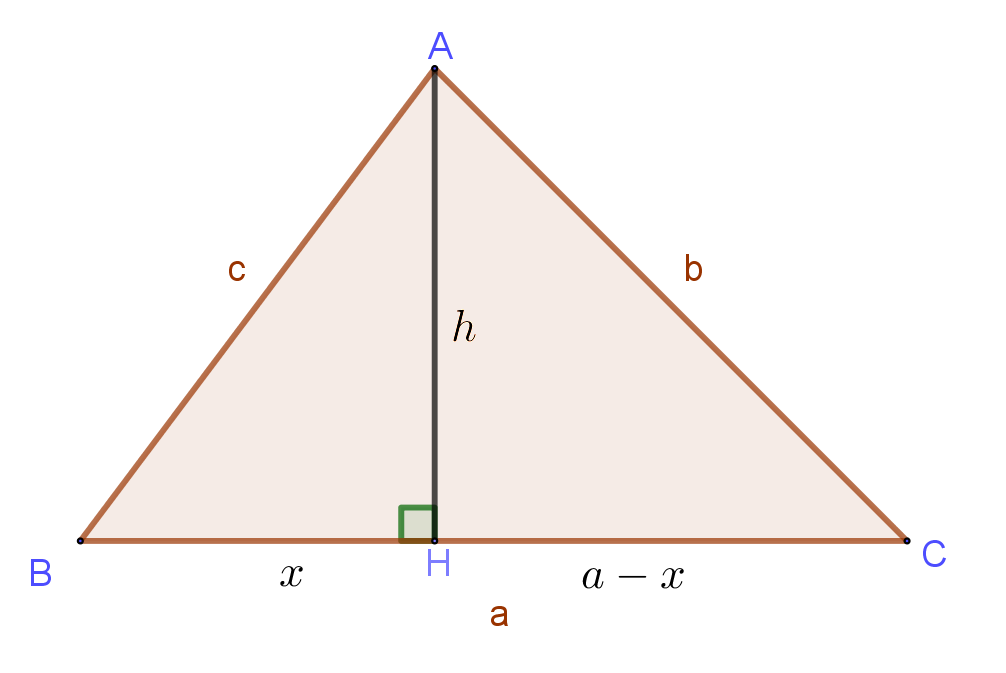
\includegraphics[width=.5\textwidth]{heron}
\end{center}
위의 그림처럼 꼭짓점 \(A\)에서 선분 \(BC\)에 내린 수선의 발을 \(H\)라고 하자.
\(\ov AH=h\), \(\ov BH=x\)라고 두면 \(\triangle ABH\)에서
\[h^2=c^2-x^2\]
이고 \(\triangle ACH\)에서
\[h^2=b^2-(a-x)^2\]
이다.
따라서
\[c^2-x^2=b^2-(a-x)^2\]
이것을 정리하면
\[x=\frac{a^2+c^2-b^2}{2a}\tag{1}\]
\(h\)의 값을 구하면
\[h=\sqrt{c^2-x^2}
=\sqrt{c^2-\left(\frac{a^2+c^2-b^2}{2a}\right)^2}
=\frac{\sqrt{4a^2c^2-(a^2+c^2-b^2)^2}}{2a}
\]
이를 통해 \(\triangle ABC\)를 구하면
\[\triangle ABC=\frac12ah=\frac{\sqrt{4a^2c^2-(a^2+c^2-b^2)^2}}4\]
따라서
\[\triangle ABC=\frac12ah=\frac{\sqrt{(a+b+c)(-a+b+c)(a-b+c)(a+b-c)}}4\tag{2}\]
이고
\[\triangle ABC=\frac12ah=\sqrt{s(s-a)(s-b)(s-c)}\tag{3}\]
이다.

%
\prob{}
\(c^2-x^2=b^2-(a-x)^2\)으로부터 \(x=\frac{a^2+c^2-b^2}{2a}\)를 유도하여라.
\procedure{.2}

\newpage
%
\prob{}
\(4a^2c^2-(a^2+c^2-b^2)^2\)
을 인수분해하여라.
\procedure{.4}

%
\prob{}
\[
\frac{\sqrt{(a+b+c)(-a+b+c)(a-b+c)(a+b-c)}}4
=
\sqrt{s(s-a)(s-b)(s-c)}
\]
이 맞는지 확인하여라.
\procedure{.24}
\end{document}